%===================================================================================================
\section{Model Structure \& Notation}\label{mod.str}
The model aims to capture heterosexual HIV transmission among the Swati population aged 15--49.
The modelled population is stratified along five dimensions
(Table~\ref{tab:model.dims} and Figure~\ref{fig:model}), including:
2 sexes~($s$), 4 activity groups~($i$), 6 HIV states~($h$), and 5 cascade states~($c$);
the fifth dimension tracks seroconcordant HIV+ partnerships
and includes strata for each of 4 partnership types ($p$) plus 1 extra stratum
--- see \sref{foi.prop} for full details.
In total, $2 \cdot 4 \cdot (1 + 5 \cdot 5 \cdot 5) = 1008$ states are modelled,
since the cascade and partnership dimensions are only applicable to people living with HIV ($h>1$).
Two types of sex acts ($a$) are also considered.
\begin{table}[h]
  \centering
  \caption{Overview of model dimensions and stratifications}
  \label{tab:model.dims}
  \begin{tabular}{lccl}
  \toprule
  Dimension & \multicolumn{2}{c}{Index} & Strata \\
  \midrule
  Sex               & ($s$) & 1 & Heterosexual Women    \\
                    &       & 2 & Heterosexual Men      \\[1ex]
  Activity group    & ($i$) & 1 & Lowest Activity       \\
                    &       & 2 & Medium Activity       \\
                    &       & 3 & Lower Risk Sex Work   \\
                    &       & 4 & Higher Risk Sex Work  \\[1ex]
  HIV status        & ($h$) & 1 & Susceptible           \\
                    &       & 2 & Acute HIV             \\
                    &       & 3 & \cdf{500}{}           \\
                    &       & 4 & \cdf{350}{500}        \\
                    &       & 5 & \cdf{200}{350}        \\
                    &       & 6 & \cdf{}{200} (AIDS)    \\[1ex]
  ART cascade       & ($c$) & 1 & Undiagnosed           \\
                    &       & 2 & Diagnosed             \\
                    &       & 3 & On ART                \\
                    &       & 4 & Virally Suppressed    \\
                    &       & 5 & Virally Un-suppressed \\[1ex]
  Partnership types & ($p$) & 1 & Main / Spousal        \\
                    &       & 2 & Casual                \\
                    &       & 3 & Occasional Sex Work   \\
                    &       & 4 & Regular Sex Work      \\[1ex]
  Sex act types     & ($a$) & 1 & Vaginal               \\
                    &       & 2 & Anal                  \\
  \bottomrule
\end{tabular}

  \floatfoot{See footnote \ref{foot:code.note} regarding indices in the code.}
\end{table}
\begin{figure}[h]
  \begin{subfigure}{\linewidth}
    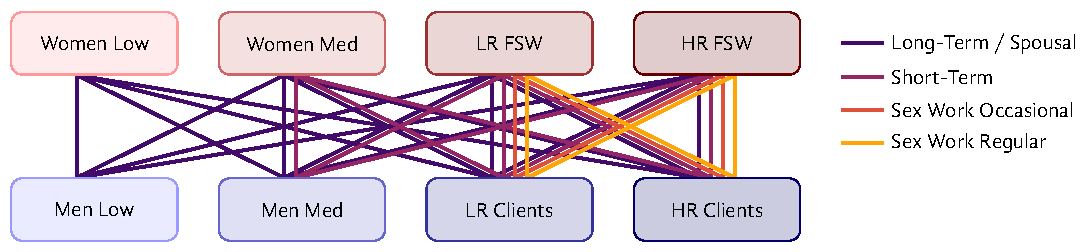
\includegraphics[scale=.8]{model.risk}
    \caption{Activity groups and partnership types}
    \label{fig:model.risk}
  \end{subfigure}
  \begin{subfigure}{\linewidth}
    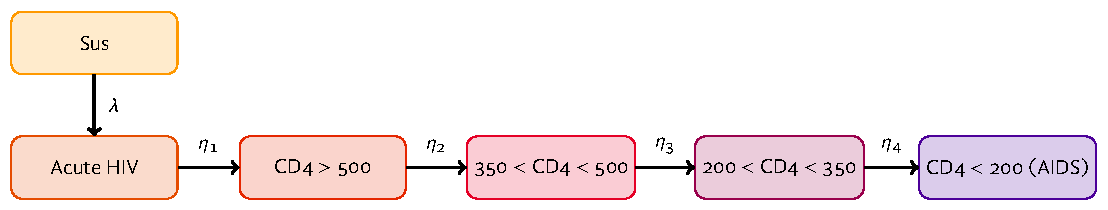
\includegraphics[scale=.8]{model.hiv}
    \caption{HIV states}
    \label{fig:model.hiv}
  \end{subfigure}
  \begin{subfigure}{\linewidth}
    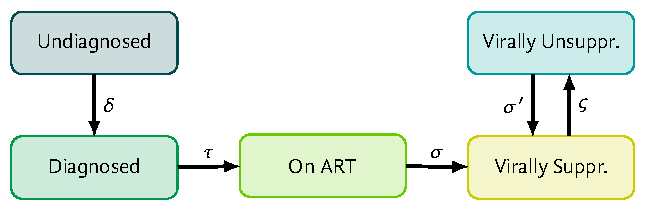
\includegraphics[scale=.8]{model.cascade}
    \caption{ART cascade states}
    \label{fig:model.cascade}
  \end{subfigure}
  \caption{Model structure and transitions}
  \label{fig:model}
  \floatfoot{
    \ffpops;
    CD4: CD4+ T-cell count per mm\tsup{3};
    Not shown: turnover amongst activity groups in \sfref{fig:model.risk}.}
\end{figure}
%---------------------------------------------------------------------------------------------------
\paragraph{Sexual Activity}
Sexual activity groups were defined to reflect common stratifications in the available data,
and persistent differences in HIV incidence and prevalence
\cite{SDHS2006,Bicego2013,Justman2016,SHIMS2}.
The lowest sexual activity group ($i=1$) comprises
individuals who had 0-1 sexual partners in the past 12 months (p12m),
but did not engage in sex work.
The medium activity group ($i=2$) similarly comprises
individuals who had 2+ sexual partners in p12m
but did not engage in formal sex work.
The highest two activity groups among women ($i=3,4$) comprise
lower and higher risk FSW (see \sref{mod.par.fsw} for more details), and
the highest two activity groups among men ($i=3,4$) likewise comprise
lower and higher risk clients of FSW.
%---------------------------------------------------------------------------------------------------
\paragraph{Partnership Types}
Four types of sexual partnerships are modelled,
capturing differences in partnership durations, and
trends in condom use relevant to inferred transmission dynamics.
The four partnership types are:
long-term/spousal partnerships ($p=1$, lowest condom use, long duration);
short-term partnerships ($p=2$, medium condom use, medium duration);
one-off/occasional sex work partnerships ($p=3$, highest condom use, 1 sex act);
and repeat/regular sex work partnerships ($p=4$, medium condom use, medium duration).
Figure~\ref{fig:model.risk} illustrates
the modelled activity groups and possible partnership types between them.
%---------------------------------------------------------------------------------------------------
\paragraph{HIV Infection \& Treatment}
HIV infection is stratified into
acute-HIV and stages defined by CD4 count (Figure~\ref{fig:model.hiv})
to reflect changes in mortality~\cite{Mangal2017},
historical ART eligibility~\cite{EswMOH2006gui,EswMOH2010gui,EswMOH2015gui,EswMOH2018gui},
and, with CD4 as a proxy for viral load, infectiousness~\cite{Boily2009}.
The modelled ART cascade (Figure~\ref{fig:model.cascade})
includes the steps associated with the ``90-90-90'' targets,
plus a generic ``virally un-suppressed'' state reflecting any combination of
treatment failure, discontinuation, or loss to follow-up after achieving viral suppression.
Loss to follow-up prior to viral suppression is not explicitly modelled,
but subsumed into rates of ART initiation and viral suppression.
